\subsection{Logging}
CentralServer har implementeret mulighed for at logge i forskellige niveauer. Der er desuden også mulighed for at skrive til forskellige slags logs.

\begin{figure}[H]
    \centering
    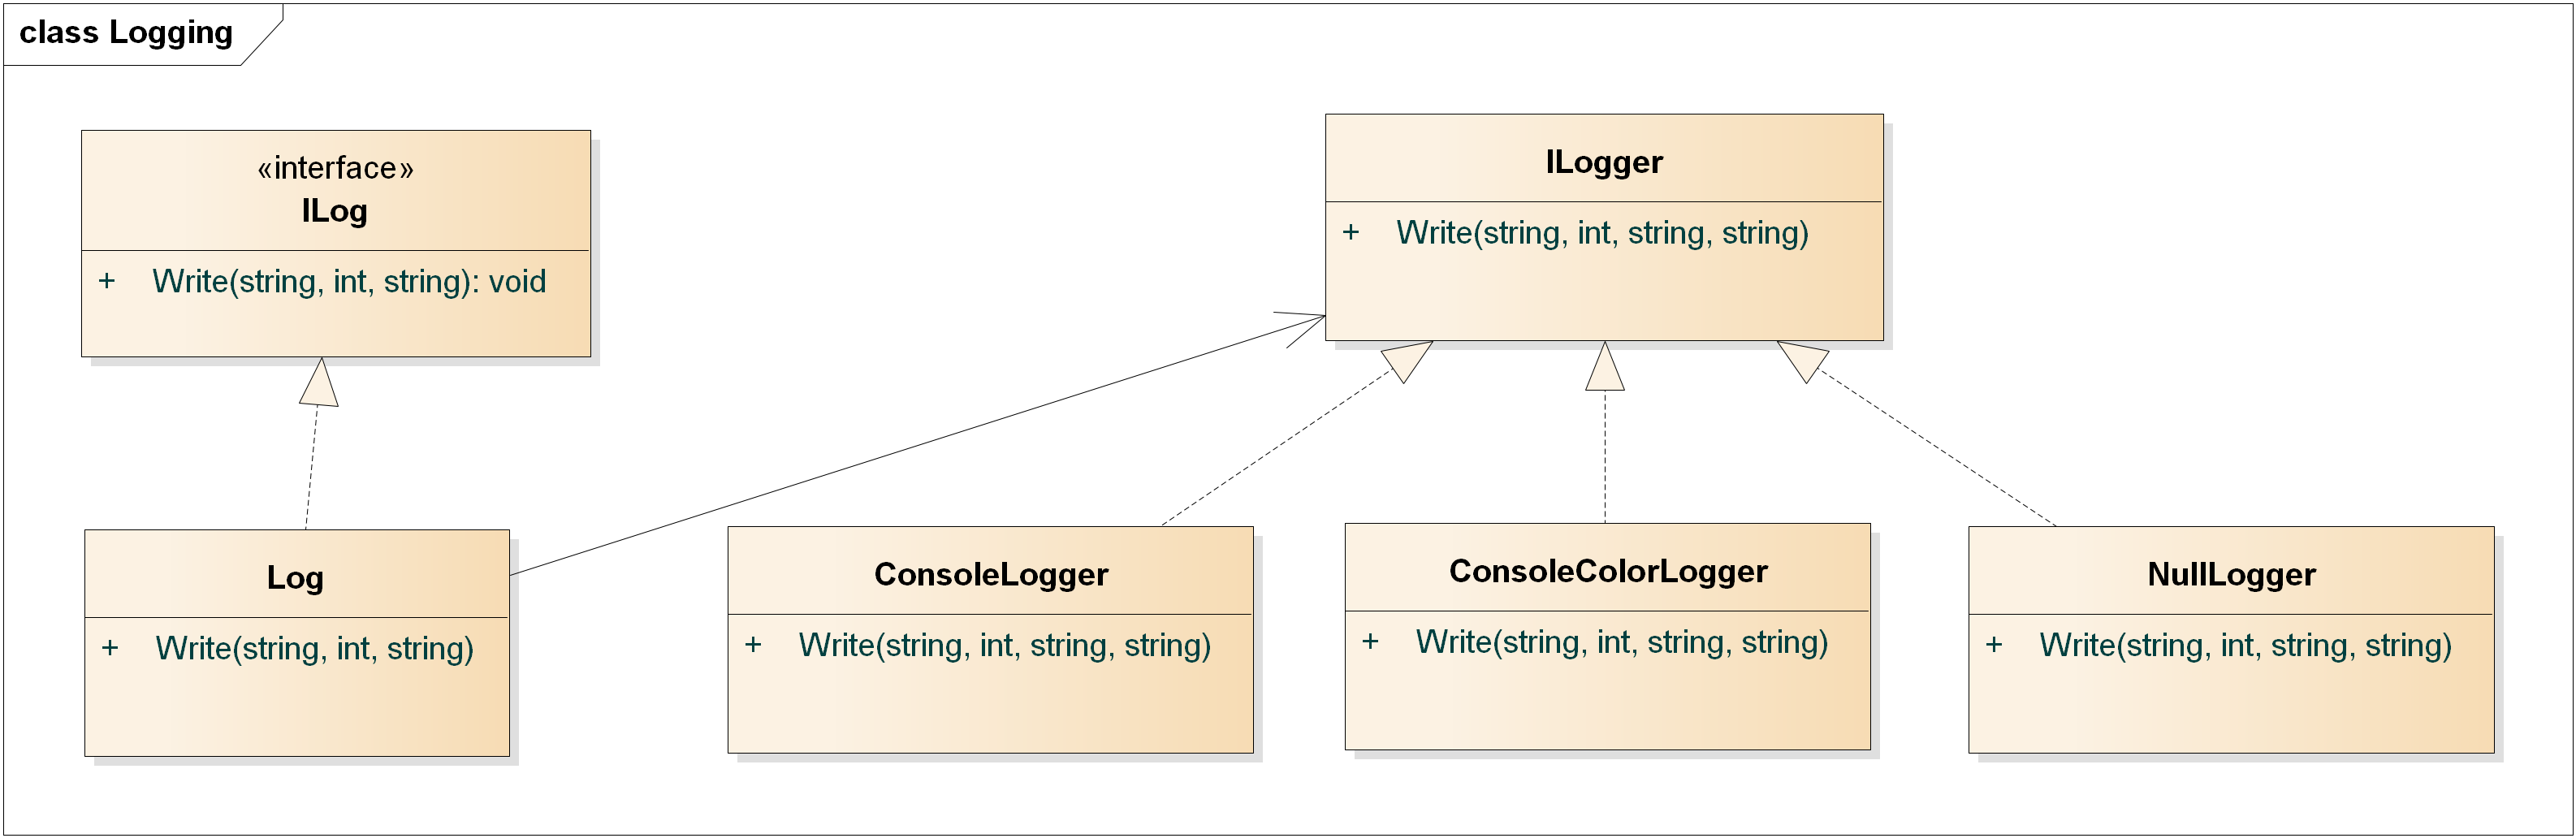
\includegraphics[width=1\textwidth]{Systemdesign/CentralServer/Images/Logging.png}
    \caption{UML-diagram for Logging pakken}
    \label{fig:CSLogging}
\end{figure}

\textbf{Niveauer}\\
Logging er delt op i flere niveauer:

\begin{itemize}
  \item Log.DEBUG (niveau 0)
  \item Log.NOTICE (niveau 1)
  \item Log.WARNING (niveau 2)
  \item Log.ERROR (niveau 3)
\end{itemize}

Når Log instantieres kan man (valgfrit) give et minimums niveau med som parameter. Alle beskeder til loggen, som er under dette niveau, ignoreres. Hvis Log eksempelvis instantieres med Log.WARNING som minimum-niveau, så vil alle beskeder med niveauerne Log.DEBUG og Log.NOTICE ignoreres. Niveau kan ikke ændres når først Log er instantieret.\\

\textbf{Loggers}\\
Når Log instantieres tager dens constructor imod et ILogger objekt. Dette objekt implementerer den lavpraktiske håndtering af, at skrive til loggen. Dette giver mulighed for nemt at implementere nye måder at logge på. Eksempelvis er logning til en fil endnu ikke implementeret, men det kan nemt gøres.\\

Følgende ILoggers er implementeret:

\begin{itemize}
  \item ConsoleLogger: udskriver til konsollen.
  \item ConsoleColorLogger: udskriver til konsollen, med farver, så der nemt kan ses forskel mellem forskellige niveauer af logging.
  \item NullLogger: gør ingenting.
\end{itemize}
